%% \begin{figure*}[!h]
%%   \centering
%%   \begin{subfigure}[t]{0.3\textwidth}
%% 	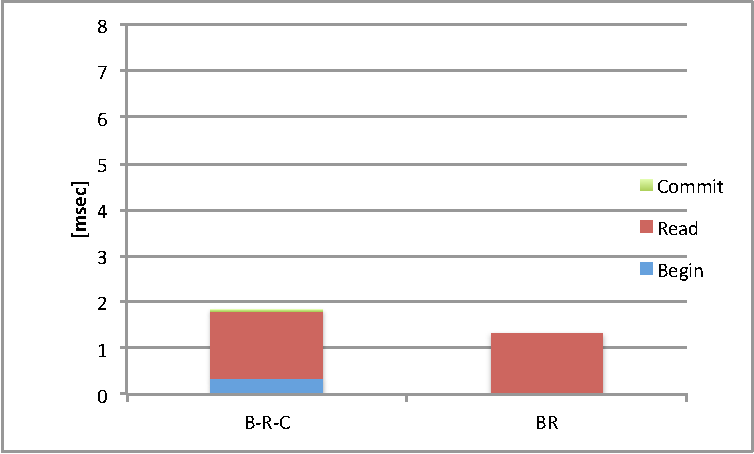
\includegraphics[width=\textwidth]{figs/read_latency.pdf}
%% 	\caption[]{Read}
%%     \label{fig:latency:read}
%%   \end{subfigure}
%%   \begin{subfigure}[t]{0.3\textwidth}
%% 	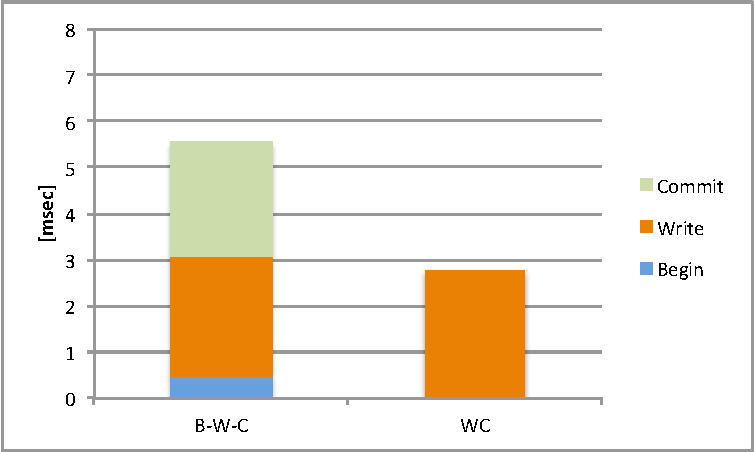
\includegraphics[width=\textwidth]{figs/write_latency.pdf}
%% 	\caption[]{Write}
%%         \label{fig:latency:write}
%%   \end{subfigure}	
%%   \begin{subfigure}[t]{0.3\textwidth}
%% 	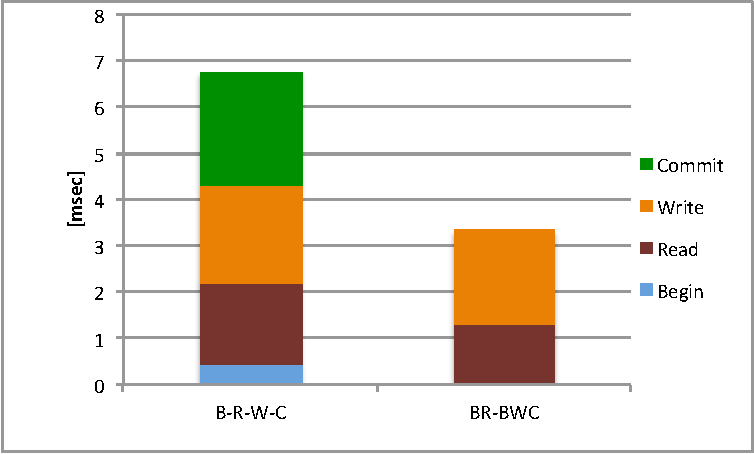
\includegraphics[width=\textwidth]{figs/rmw_latency.pdf}
%% 	\caption[]{Read Modify Write}
%%     \label{fig:latency:rmw}
%%   \end{subfigure}			
%%   \caption{Breakdown of transaction latency}
%%   \label{fig:latency}
%% \end{figure*}

\begin{figure}
\caption{Benchmark architecture that emulates a large system. The YCSB client generates complete transactions 
for a small fraction of the traffic, and measures their end-to-end latency. The custom client generates background 
begin and commit requests for the remainder of the traffic, to emulate full load on the TM.}
\label{fig:experiment}
\end{figure}

\begin{figure*}[t]
  \centering
  \begin{subfigure}[t]{0.33\textwidth}
	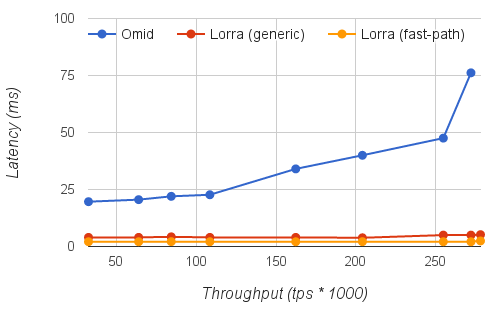
\includegraphics[width=\textwidth]{figs/thpt-latency-1.png}
	\caption[]{Transaction size = 1}
         \label{fig:tl-1}
  \end{subfigure}
  \begin{subfigure}[t]{0.33\textwidth}
	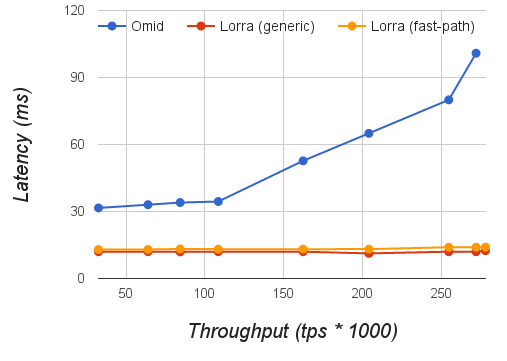
\includegraphics[width=\textwidth]{figs/thpt-latency-5.png}
	\caption[]{Transaction size = 5}
    \label{fig:tl-5}
  \end{subfigure}
    \begin{subfigure}[t]{0.33\textwidth}
	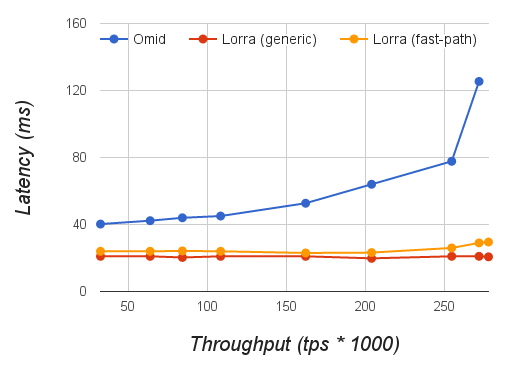
\includegraphics[width=\textwidth]{figs/thpt-latency-10.png}
	\caption[]{Transaction size = 10}
    \label{fig:tl-10}
  \end{subfigure}			
  \caption{{\sys} (generic and FP API's) versus Omid, in terms of latency and throughput. Transactions are considered
by size (1, 5, and 10 data accesses). }
  \label{fig:throughput-latency}
\end{figure*}

\begin{figure*}
  \centering
  \begin{tabular}{cccc}
    
  \begin{subfigure}[t]{0.4\textwidth}
	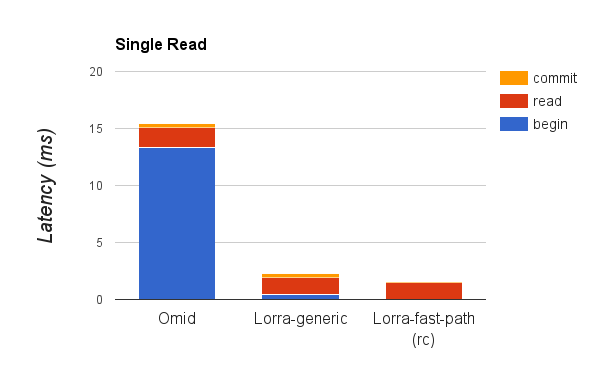
\includegraphics[width=\textwidth]{figs/stack-brc.png}
	\caption[]{Single-write transactions}
    \label{fig:stack-brc}
  \end{subfigure} &

  \begin{subfigure}[t]{0.4\textwidth}
	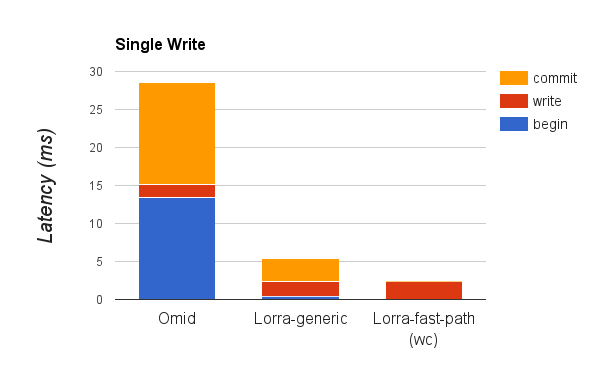
\includegraphics[width=\textwidth]{figs/stack-bwc.png}
	\caption[]{Single-read transactions}
    \label{fig:stack-bwc}
  \end{subfigure} \\

    \begin{subfigure}[t]{0.4\textwidth}
	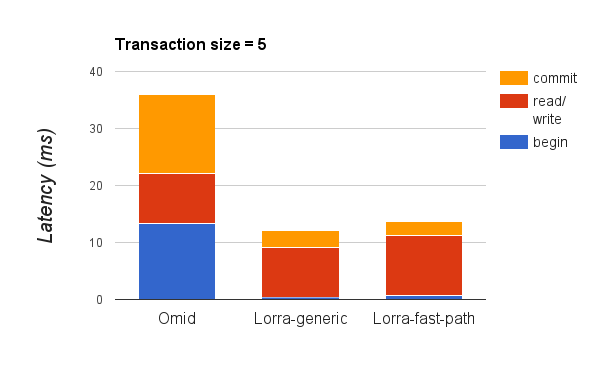
\includegraphics[width=\textwidth]{figs/stack-tx5.png}
    \caption[]{Transaction size = 5}
    \label{fig:stack-tx5}
  \end{subfigure} &

  \begin{subfigure}[t]{0.4\textwidth}
	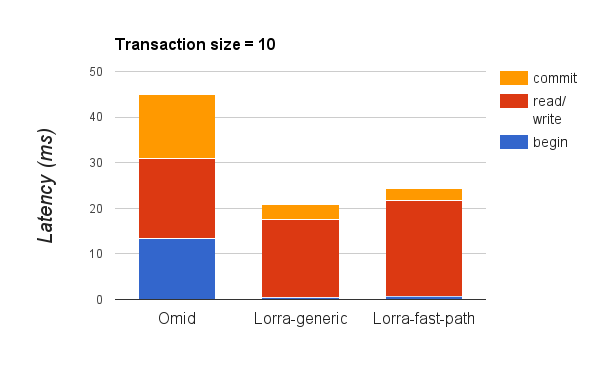
\includegraphics[width=\textwidth]{figs/stack-tx10.png}
    \caption[]{Transaction size = 10}
    \label{fig:stack-tx10}
  \end{subfigure} \\
  
  \end{tabular}
  \caption{Zoom-in on latency breakdown in specific scenarios, under the 100K tps workload.}
  \label{fig:zoomin}
\end{figure*}

We evaluate {\sys}'s performance for both the generic and the fast-path transactions, 
in terms of average transaction latency under a variety of workloads. We compare {\sys\/} 
(the generic and fast-path API's) to the mainstream Omid implementation. Both {\sys\/} 
and Omid use HBase as KV-storage backend. Both are configured for low-latency asynchronous 
post-commit.   

We run the experiments on 12-core Intel Xeon 5 machines with 46GB RAM and 4TB 
SSD storage, interconnected by 1G Ethernet.  Every node runs the HBase and the underlying 
Hadoop filesystem (HDFS) serving tiers within 8GB JVM containers. 

\subsection{Methodology}
We project the transaction performance in a very large production KV-store in which the data (read/write) 
requests are roughly load-balanced. To this end, horizontal scaling of the KV-store and its workload do not 
affect the performance of the data requests. The control (begin/commit) requests are served by the centralized 
TM; scaling the workload congests this bottleneck. We can therefore capture the end-to-end transaction latency
in the projected system with a small HBase cluster that serves a fraction of workload, while stressing the TM 
by a full load of control requests. 

We emulate a 1000-node HBase with a 3-server cluster that processes $0.3\%$ of the projected workload. 
This traffic is driven by the popular YCSB benchmark~\cite{Cooper:2010:BCS:1807128.1807152} 
that exercises the traditional (synchronous) transaction processing API. YCSB measures the end-to-end latencies.
The remainder of the control requests (background load on the TM) are generated by a custom tool~\cite{Omid2017} 
that asynchronously posts them on the wire, and collects the TM responses. Both workload
drivers exploits up to 3 client nodes. Figure~\ref{fig:experiment} depicts the experiment's architecture. 

Our test cluster stores approximately 23M keys, which amounts to 7.66B keys in the emulated system. 
The values are 2K big, which translates to roughly 46GB data, replicated three-way in HDFS. The keys are hash-partitioned
across the servers, thereby balancing the amount of data governed by each server. The data accesses are 50\% reads and 
50\% writes. The key access frequencies follow a Zipf distribution, generated following the description in~\cite{Gray:1994:QGB:191839.191886}. 
The Zipf parameter is $\theta=0.8$ (derived from production workloads). The resulting distribution is very heavy-tailed, which 
guarantees that neither of the servers suffers an excessive portion of traffic due to super-popular items, i.e., the 
data requests are load-balanced, similarly to the data itself.  

Transaction sizes (number of reads and writes) follow a Zipfian distribution with $\theta=0.99$, with a cutoff at 10. 
In this context, 63\% of the transactions access 3 keys or less, whereas 3\% access 10 keys. The system loads
vary from 30K to 300K transactions per second (tps). 

\subsection{Numerical Results} 

We start by studying the system performance in throughput-latency terms. 
Within the workload mix described above, we compare the end-to-end latencies by transaction class -- 
1, 5, and 10 data accesses. Figure~\ref{fig:throughput-latency} depicts the results, for the three systems. 

Both {\sys\/} implementations are ubiquitously faster than Omid. {\sys\/} exhibits lower latencies under light loads, 
thanks to its reduction in commit network trips. For example, single-key transactions complete on average within 
5ms under {\sys}'s generic API, versus Omid's 20ms. For longer transactions, the gap remains fixed but is amortized 
by other operations. Under high loads, {\sys\/} scales almost perfectly whereas Omid suffers from a well-pronounced 
bottleneck. For instance, Omid's single-key transaction latency soars to 75ms for under 300K tps whereas
{\sys}'s remains almost flat. The extra delay in Omid is due to commit table write batching, which its TM applies 
to handle congestion~\cite{Omid2017}. %In comparison with Omid, the differences between {\sys}'s flavors are negligible. 

We now zoom-in on the latency of the three TPSs, under a moderate load of 100K tps. Namely, we dissect the end-to-end 
transaction latency to its begin, read/write, and commit components. Figure~\ref{fig:zoomin} illustrates the breakdown. 
With Omid, the control requests dominate the delay: 94\% for single-write, 89\% for single-read, and 61\%
even for 10-access transactions! Note that Omid's begins are no less expensive than commits because both 
requests get blocked on commit table writes. 

TBD 

\remove{

\paragraph{FP API latency}
Figure~\ref{fig:latency} compares the latency observed by YCSB when running regular and FP transactions.
We focus on 3 types of transactions: (1) Read, (2) Write and (3) Read modify write.

Figures~\ref{fig:latency:read} and \ref{fig:latency:write} show the latency of a single read and write transaction. Regular transactions (b-r-c, b-w-c) query the TSO at the begin and commit stage which add 0.3ms for read transactions and 3ms for write transactions.
Figure~\ref{fig:latency:rmw} compares the latency of a read modify write transaction, once using the FP API (br-bwc) and once using the regular transaction API (b-r-w-c).The begin and commit stage of the regular transaction add 3ms to each transaction.
}





\remove{
\Yoni{
  --background noise
  --switch order of charts
  --explain that the LL is better for all TPS so it doesn't matter the point we choose to check}
}